\documentclass{report}

\title{Forest Road Simulation using OpenGL}
\date{2021-08-24}
\author{Nishan Poudel \and Smaran Dhungana \and Sukriti Subedi}

\usepackage[utf8]{inputenc}
\usepackage{graphicx}
\usepackage{setspace}
\setstretch{1.5}
\usepackage{geometry}



\begin{document}

\begin{center}
\thispagestyle{empty}
\LARGE{Tribhuvan University}\\[-0.9ex]
\LARGE{Institute of Engineering, Pulchowk Campus}\\[2ex]
\large{Department of Computer and Electronics Engineering}\\
\vspace{0.3cm}
\begin{center}

\includegraphics[width=7cm]{tu.png}\\
\vspace{0.5cm}
\textbf{\Large{A Project Report on:}}\\
\medskip\par
\textbf{\LARGE{Forest Road Simulation using OpenGL}}
\medskip\par
\vspace{0.7cm}
\Large{\textbf{Submitted to:}}\\[-0.5ex]
\large{Prof. Anil Verma}\\[-1.5ex]
\large{Department of Computer Engineering}
\bigskip\par
by \par
\large{Nishan Poudel }\\[-1ex]
\large{075BCT057}\\ [-1ex]
\vspace{0.6cm}
\large{Smaran Dhungana }\\[-1ex]
\large{075BCT086}\\ [-1ex]
\vspace{0.6cm}
\large{Sukirti Subedi }\\[-1ex]
\large{075BCT089}\\ [-1ex]
\vspace{0.6cm}
\large{ Submission Date: }\\[-1ex]
\large{\today}
\vspace{0.6cm}
\end{center}
\end{center}


\maketitle

\tableofcontents
\listoffigures

\begin{abstract}
    Since the advent of powerful GPUs, video games have been made more realistic using stunning background 
    made using Computer graphics. In this project, we've tried to implement our own graphics model of forest 
    roadside environment using OpenGL. The individual elements of the scene were first designed using an open
    -source 3D modeling tool called Blender. Then the graphics model was imported onto OpenGL environment 
    using a wavefront (.obj) extension and we focused on implementing the classic algorithms used in Computer
    Graphics including transformations, lighting and rasterization. We experimented using different projections, 
    camera angles, colors, shading methods and finally came to the decision as evident in our project demo.
    The models were then polished using some 
    manually selected textures and at the end the whole scene was fitted inside a skybox to create the illusion 
    of an open sky in the scene. Also, we experimented with a night mode for the whole scene by changing
    lighting configurations and skybox textures.
\end{abstract}

\section{Introduction}

    Our project titled 'Forest Road Simulation' is an attempt to create a 3D Graphical environment as a 
    way to incorporate all the things we've learned about Computer Graphics. As the title suggests, the 
    main scene of our project consists of a Road, fences on one side, sparse trees on either side, a small
    hill and the whole landscape is surrounded by a wide open sky. The user is supposed to move in a 
    single direction in the scene along the road. Only the hill is at a certain elevation above the rest 
    of the elements of the scene. Most of the trees present in the scene are of uniform height. The road 
    is purposedly made zigzag so as to make the scene more realistic as possible. The light source is located 
    above the scene as indicated by the skybox. As the scene was created in Blender, the whole scene can 
    be divided into a number of meshes. The meshes are mainly of five types:
    \\i) Trees 
    \\ii) Road 
    \\iii) Fences 
    \\iv) Land 
    \\v) Hills

\subsection{Background}
    Since our project's main goal was to learn about Graphics Programming, we didn't have much knowledge 
    about different concepts used to create Computer Graphics. Most of the things, we learned along the way 
    and kept on implementing the newly learned things. Our knowledge in linear algebra, trigonometry, C++ 
    and some basic graphics skills such as photo editing were very helpful. Computer graphics deals with 
    a lot of matrices to render visuals and all of the algorithms for the efficient graphics calculations 
    were based on the foundations of vector operations such as transformations, mulitply, addition etc. The 
    project also needed above-average programming skills to write all the necessary program modules needed 
    to implement the idea. We worked with many programming concepts such as File handling, Operator overloading, 
    String manipulation etc. The programming mode is mostly procedural but some libraries required some knowledge 
    of Object Oriented Programming as well. This project also required the background of fluency in mathematical 
    visualizations to better understand graphics operations and communicated with project teammates.
\subsection{Objectives}
    Our main objective was to implement all the transformations, shading, lighting and buffer algorithms within 
    the scope of our project idea. We wanted to create a realistic scene using all the concepts we learned and 
    decided that crearing an outdoor scene simulation would be the best way to meet all our objectives. Our main 
    objectives regarding the project were:
    \medskip
    \\1.  To implement basic Computer Graphics algorithms.
    \\2.  To learn about graphics programming using OpenGL.
    \\3.  To learn about 3D modeling and import the 3D models in OpenGL.
    \\4.  To understand the complexity involved in rendering realistic scenes.
    \\5.  To know more about state-of-the-art graphics methods.
    \\6.  To experiment with best lighting and shading configurations and with best possible positions and 
    angles for the camera. 
\subsection{Motivation}
    Computer Graphics is a very vast field and there are other myriad ideas that we could've worked on. 
    After a lot of brainstorming, we decided to go with this project idea as we saw that it was perfect to 
    implement all the concepts we knew and the end goal seemed very tempting to us. We got the inspiration for 
    the project idea from the popular racing games and other Role Playing Games(RPGs) such as Roadrash, Asphlant, 
    GTA etc. All of these games use very minimalistic yet realistic looking graphics backgrounds. So, we decided 
    to create a similar scene for our project. We also took a look at different other graphics creations on the 
    internet to decide on a clear end-goal before proceeding with the project. This image was the one we 
    decided to take as reference.
    \medskip
    \begin{figure}[h!]
      \centering
        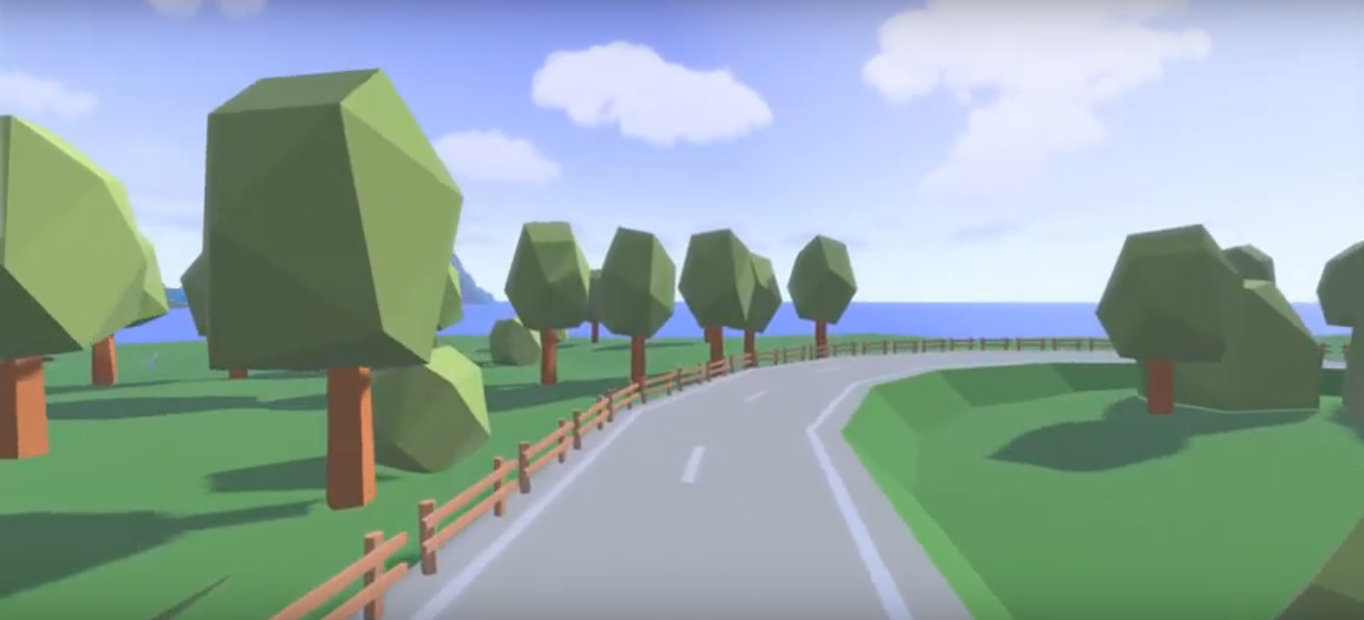
\includegraphics[width=8cm,height=10cm,keepaspectratio]{motivation.png}
        \caption{Reference scene.}
    \end{figure}
\subsection{Scope}
    Computer Graphics is a vastly deep and complex field and there were endless things that we could've done 
    but we decided to focus on only the important bits. Since the inception of the project idea, we thought of 
    this project as a background scene of a video game. So, this model could be easily integrated with a racing 
    or a similar type of game coded using C/C++. Since the scene requires lighting, there were many choices for 
    shading/light reflection models such as Phong Reflections etc. Similarly, out of shading interpolation methods such as 
    Gourard, Phong etc, anyone of them could be used. We could've gone with Orthograpic projections but it 
    didn't seem that realistic that using Perspective projection. We also implemented Depth testing using 
    Z-buffer algorithm in the project. There was also scope for implementing shadows either by baking them 
    in the textures or using Shadow Mapping. The first one seemed really inflexible and the second one needed 
    extra time and effort. So, we weren't able to include shadows in our project.

\section{Literature Review}
\subsection{Introduction}
The advent of Computer Graphics is intertwined with the advent of Modern Electronic Computers. The computer graphics which
we associate, today with the photo realistic Video game had very humble beginning with a simple CRT monitor where electron dot were
projected to create a line. In today's world the Computer graphics is the single most widely used technology, which is almost inevitable for us Human
to operate our society. It is crucial in all part of human activity as almost all our work these days is digitized and digital system
display things in screen not in log book.

\subsection{Related Theories and Technologies}
In the 1950s the Been Laposky displayed the oscilloscope graphic generated by analog electronic machine, which is considered as the first
graphics image on a display. Of course, the technology was simple compared to today's sophisticated rendering techniques, it used electron beam
manipulation to achieve the imagery. Subsequently, in 1951 UNIVAC-I was developed with real time video display capable of displaying real time text and graphic on
oscilloscope screen. Now in the 1960s the field is maturing and the term Computer Graphics was coined in same year by William Fetter. Space Wars(first computer video game)
was made by Stove Russel in consequent year. Similarly, in 1963 Douglas Englebart developed first mouse, 1964 William Fetter developed computer model of human figure, and  in 1954 Jack Bresenham
developed the infamous line drawing algorithm. Moving on, the first subdivision algorithm, hidden surface algorithms was developed with bell lab
introducing first frame buffer containing 3 bits per pixel. Now more advanced application with computer graphics was being possible. Applications
like automated drafting with CAD, computer aided manufacturing were is introduced to the market.

Entering to early 70s, improvement were made in raster display technology and in 1972 Nolan Kay Bushnell made video arcade game while year before that the Gourand Shading rendering model was developed and subsequently the
Phong Shading rendering model was released to world. While the graphics system were being advanced day by day, parallelly the way to utilize those technologies too. Now the artist were
using the computer graphics to produce their art product and filmmakers were using computer graphics to enhance the effect of scene in movie to
creating an entire movie sequence digitally. Fast-forward to 1995s, the first full length computer generated feature film "Toy Story" was made.
During the period of 70s to 90s a lot of new technology and improvement were made, which made the Toy Story possible among such technologies includes, the color graphics personal computer
Apple II, raster graphic, bitmap image, Ray Tracing Rendering model, Polhemus (first 3D graphics software), VGA and SVGA technology and many others.

\subsection{Related Works}
The 2021's century is here, the century of technology and human prosperity where the computer, hence the computer graphics is
pivotal piece to this puzzle of continuous innovation in technology. In modern days, print design, digital art, special effects, the video games
and visuals effects all are powered by the computer graphics. The field is so vast that it, have given birth to many independent branches
of studies such as Computational geometry, Computational topology, Computer vision, Image Processing,  Information Processing and Scientific Visualization.
With such a wide open  slate for exploration, the computer graphics is still evolving and innovating. The new technology like
holographic projection, virtual reality, augmented reality and real-world biological simulation are still in their infancy.
The field itself is in upper echelon of maturity, but in future the development would be geared more towards Computer graphics as
Enabler technology for other domain to develop and innovate than itself, for instance using computer graphics to develop more effect drug distribution,
modeling the human body for efficient surgery and many others.

\subsection{Conclusion}

In this way, the humble beginning of computer graphics is now the pivotal piece of human existence. It enabled
us to do task which were previously difficult or impossible. It makes the digital revolution possible and propelled the humanity to new
arena of innovation and development. Furthermore, it made other technology to flourish in rapid pace, made our society more efficient and productive as it
eliminated the need for physical communication with paper and other means with digital displays.
Overall, it is one of the most important tool developed by human being along with the computer itself.



\section{Methodologies}
    We first started with Blender to build the 3D Representation of our model. We crafted different 3D models 
    for tree, road, fences, hill and land. Then they we all put together into a single (.blend) file in the 
    Blender software. Blender also has features of baking textures onto models and exporting them into other 
    file formats. The textures were exported into (.DDS) file formats accordingly and put into the project 
    codebase. After that the we began writing programs using the OpenGL library(GLEW) to import the model created 
    using Wavefront(.obj) file format. Implementations of Lighting, Shading and Transformations were then implemented. 
    \\The project workflow can be understood as:
    \medskip
    \\1.    Create 3D Model using Blender. 
    \\2.    Importing models and textures in OpenGL. 
    \\3.    Implementing all the Graphics Algorithms. 
    \\4.    Configure Camera, Lighting, Projections etc. 
    \\5.    Compile and test the Codebase.
\subsection{Graphical Representation}
    During 3D Modeling of our objects, they could be represented in different kinds of views. In Wireframe 
    representation, we get to see the suraces of scenes approximated using many small triangles and quadrilaterals. 
    Wireframe models are supposed to show the models form a geometrical point of view. This way, it became a lot 
    easier for us to create the 3D Models by thinking of all those complex shapes in the scenes as simple combinations 
    of planar surfaces. After that, we see the material representation of the scene. This is how we'll represent the 
    scene in its final form but accurate textures will be applied onto the surfaces instead of arbitary colors. 
    Then we see the view port representation of the scene. Here, each surface in the scene is supposed to have its 
    own normal direction and this dictates the effect of light source on the color component of the surface.

    \medskip
    \begin{figure}[h!]
      \centering
        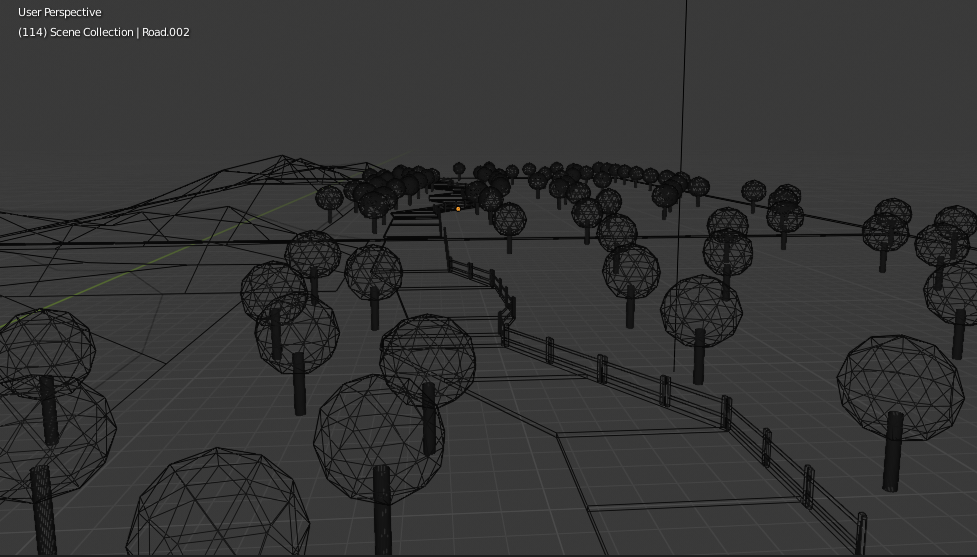
\includegraphics[width=12cm,height=12cm,keepaspectratio]{development-wireframe.png}
        \caption{Wireframe Representation}
    \end{figure}
    \medskip
    \begin{figure}[h!]
      \centering
        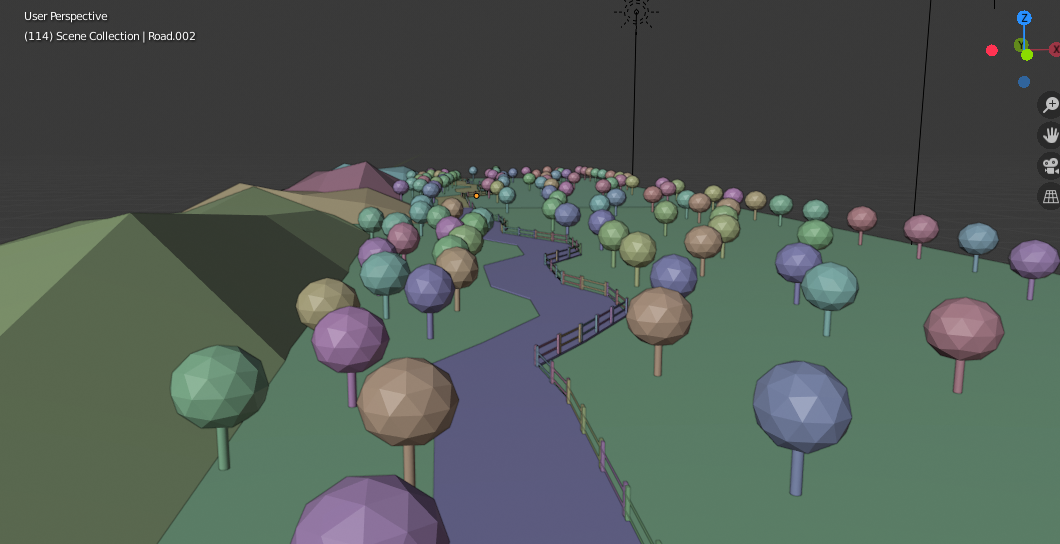
\includegraphics[width=12cm,height=12cm,keepaspectratio]{development-material.png}
        \caption{Material Representation}
    \end{figure}
    \medskip
    \begin{figure}[h!]
      \centering
        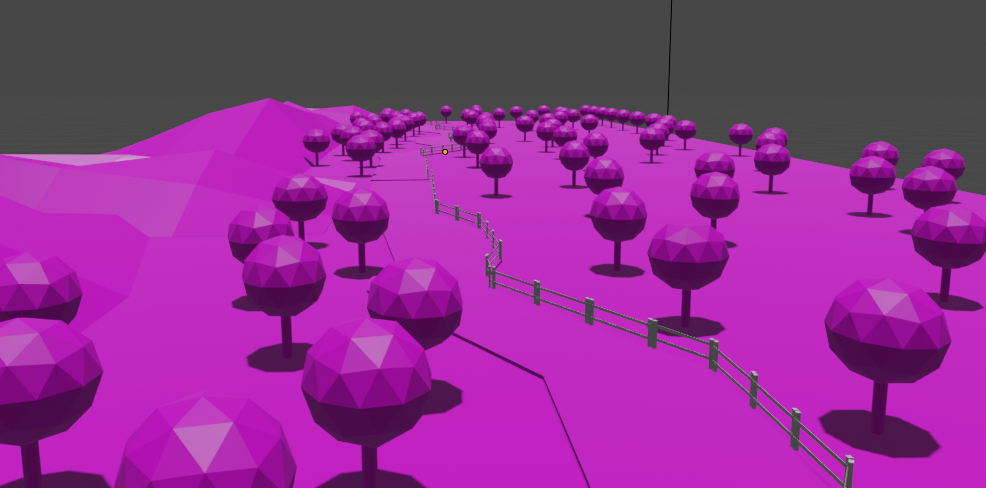
\includegraphics[width=12cm,height=12cm,keepaspectratio]{development-shading.png}
        \caption{Viewport Representation}
    \end{figure}

\subsection{Algorithms and Implementations}
    \paragraph{Viewing Pipeline}
         The graphics pipeline consists of three conceptual stages. Depending on the implementation, all parts may be done by the CPU or parts of the pipeline may be done by an accelerator card. The conceptual model is useful in either case: it helps you to know where your application spends its time. The stages are:

    The application. The application program running on the CPU, feeding commands to the graphics 
    subsystem (always on the CPU).
    The geometry subsystem. The per-polygon operations, such as coordinate transformations, lighting, 
    texture coordinate generation, and clipping (may be hardware-accelerated).
    The raster subsystem. The per-pixel operations, such as the simple operation of writing color 
    values into the framebuffer, or more complex operations like depth buffering, alpha blending, and 
    texture mapping (may be hardware accelerated). 

    \medskip
    \begin{figure}[h!]
      \centering
        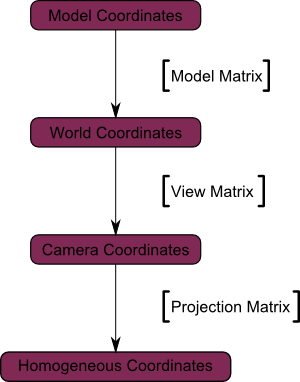
\includegraphics[width=6cm,height=6cm,keepaspectratio]{pipeline.png}
        \caption{3D Viewing Pipeline}
    \end{figure}

The amount of work required from the different pipeline stages varies depending on what the application does. For example, consider a program that draws a small number of large polygons. Because there are only a few polygons, the pipeline stage that does geometry operations is lightly loaded. Because those few polygons cover many pixels on the screen, the pipeline stage that does rasterization is heavily loaded
    \paragraph{Transformations}
        3D rotation is not same as 2D 
        rotation. In 3D rotation, we have to specify the angle of rotation along with the axis of 
        rotation.
        You can change the size of an object using scaling transformation. In the scaling process, 
        you either expand or compress the dimensions of the object. Scaling can be achieved by 
        multiplying the original coordinates of the object with the scaling factor to get the desired 
        result. 
        A transformation that slants the shape of an object is called the shear transformation. Like in 
        2D shear, we can shear an object along the X-axis, Y-axis, or Z-axis in 3D.
        Transformation matrix is a basic tool for transformation. A matrix with n x m dimensions is
        multiplied with the coordinate of objects. Usually 3 x 3 or 4 x 4 matrices are used for 
        transformation
    \paragraph{Projection}
    Perspective projection or perspective transformation is a linear projection where three dimensional 
    objects are projected on a picture plane. This has the effect that distant objects appear smaller 
    than nearer objects.\cite{DUMMY:1}

    It also means that lines which are parallel in nature (that is, meet at the point at infinity) 
    appear to intersect in the projected image, for example if railways are pictured with perspective 
    projection, they appear to converge towards a single point, called the vanishing point. Photographic 
    lenses and the human eye work in the same way, therefore perspective projection looks most 
    realistic. Perspective projection is usually categorized into one-point, two-point and 
    three-point perspective, depending on the orientation of the projection plane towards the axes of 
    the depicted object.
    \medskip
    \begin{figure}[h!]
      \centering
        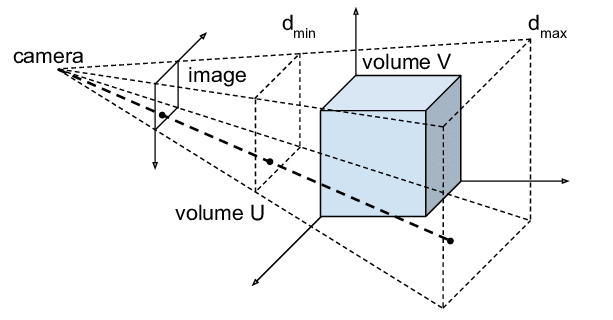
\includegraphics[width=6cm,height=6cm,keepaspectratio]{perspective.png}
        \caption{Perspective Projection}
    \end{figure}

    \paragraph{Depth Testing (Z Buffer):}
    A depth buffer, also known as a z-buffer, is a type of data buffer used in computer graphics to 
    represent depth information of objects in 3D space from a particular perspective.\cite{DUMMY:3} Depth buffers are 
    an aid to rendering a scene to ensure that the correct polygons properly occlude other polygons.
    n a 3d-rendering pipeline, when an object is projected on the screen, the depth (z-value) of a generated 
    fragment in the projected screen image is compared to the value already stored in the buffer (depth 
    test), and replaces it if the new value is closer. It works in tandem with the rasterizer, which 
    computes the colored values. The fragment outputted by the rasterizer is saved if it is not overlapped 
    by another fragment. 
    \medskip
    \begin{figure}[h!]
      \centering
        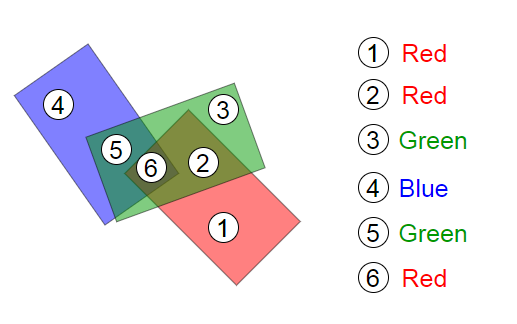
\includegraphics[width=6cm,height=6cm,keepaspectratio]{z-buffer.png}
        \caption{Z-Buffer Illustration}
    \end{figure}

    \paragraph{Shading and Light Reflection Model: Phong}
    Phong shading is an interpolation technique for surface shading invented by the computer graphics 
    pioneer Bui Tuong Phong. It is also called Phong interpolation, or normal-vector interpolation 
    shading. It interpolates surface normals across rasterized polygons and computes pixel colors 
    based on the interpolated normals and a reflection model. Phong shading may also refer to the 
    specific combination of Phong interpolation and the Phong reflection model.\cite{DUMMY:2} 

        Phong shading may also refer to the specific combination of Phong interpolation and the Phong 
    reflection model, which is an empirical model of local illumination. It describes the way a surface 
    reflects light as a combination of the diffuse reflection of rough surfaces with the specular 
    reflection of shiny surfaces. It is based on Bui Tuong Phong's informal observation that shiny 
    surfaces have small intense specular highlights, while dull surfaces have large highlights that 
    fall off more gradually. The reflection model also includes an ambient term to account for the 
    small amount of light that is scattered about the entire scene. 

    \medskip
    \begin{figure}[h!]
      \centering
        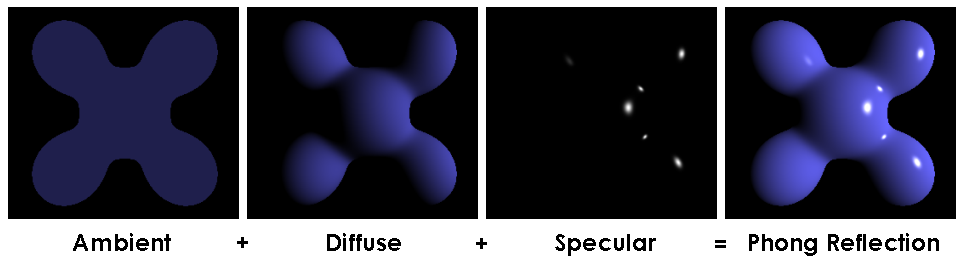
\includegraphics[width=12cm,height=12cm,keepaspectratio]{Phong4.png}
        \caption{Phong Reflection Model}
    \end{figure}

    \medskip
    \begin{figure}[h!]
      \centering
        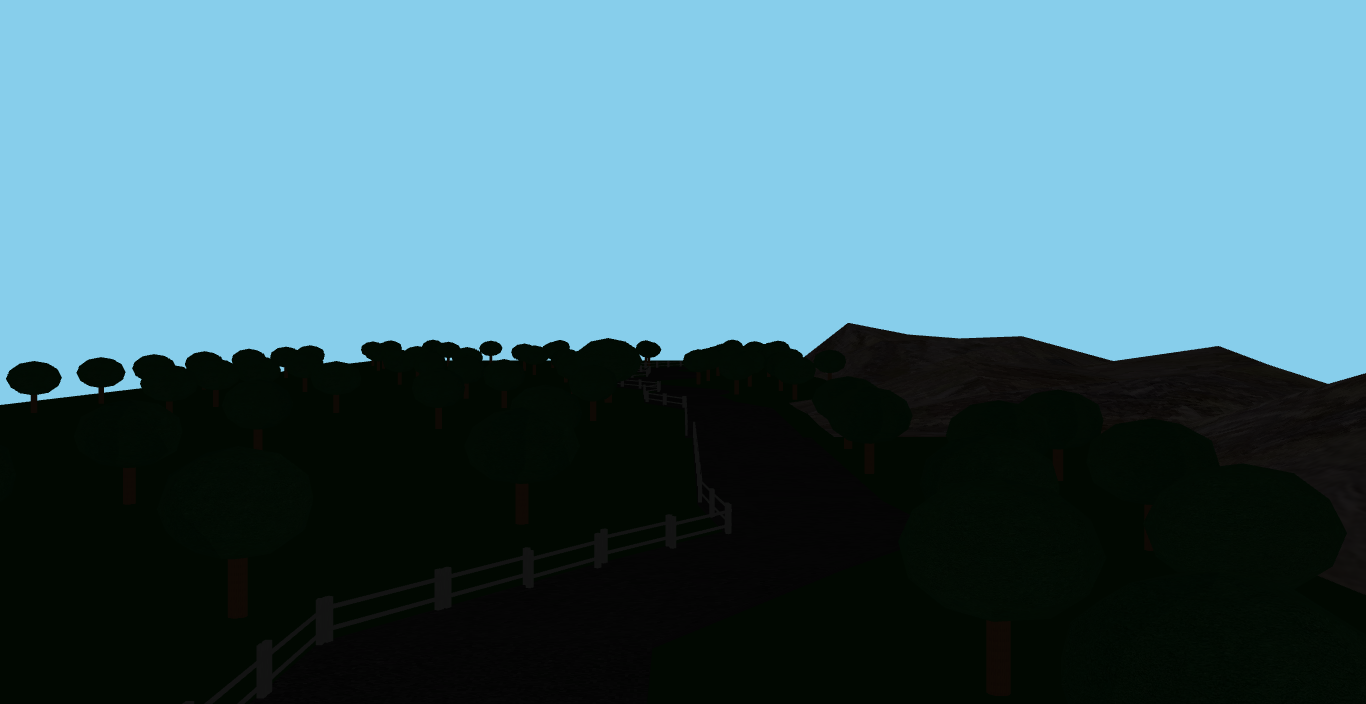
\includegraphics[width=10cm,height=10cm,keepaspectratio]{ambient.png}
        \caption{Ambient Lighting}
    \end{figure}

    \medskip
    \begin{figure}[h!]
      \centering
        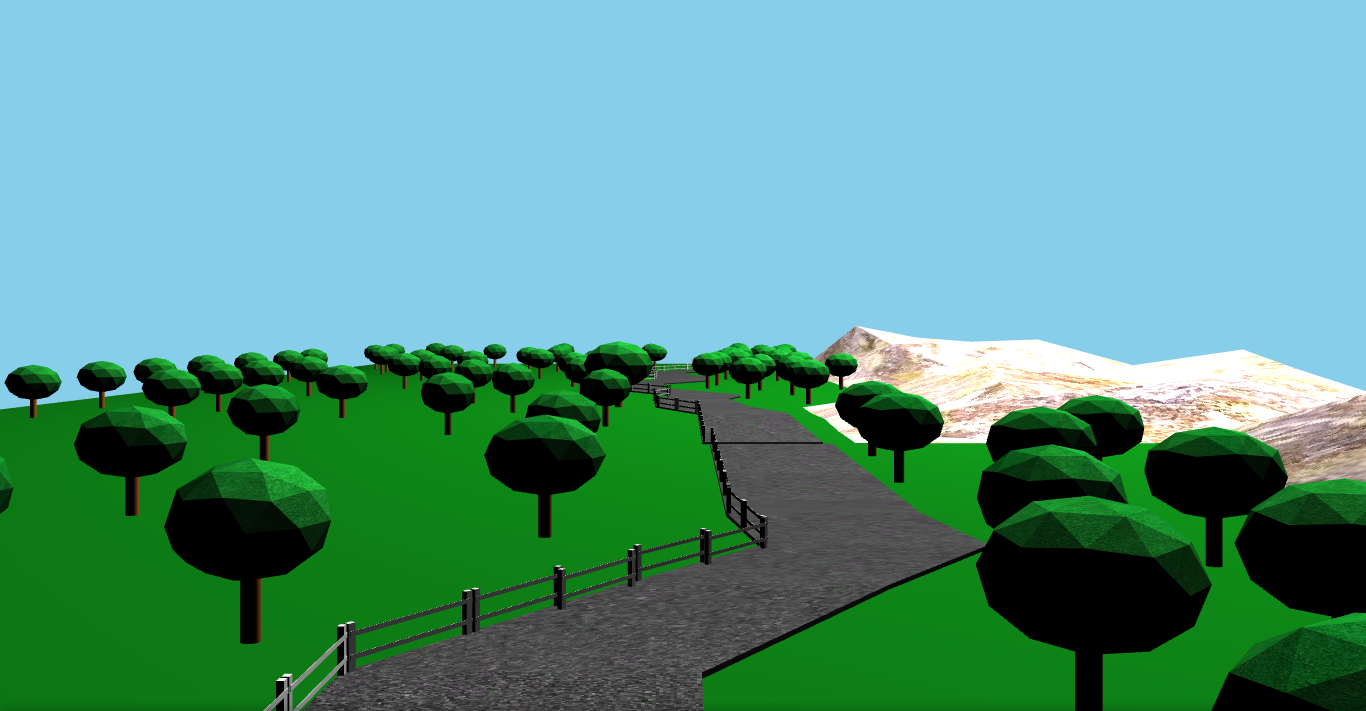
\includegraphics[width=10cm,height=10cm,keepaspectratio]{diffuse.png}
        \caption{Diffuse Lighting}
    \end{figure}

    \medskip
    \begin{figure}[h!]
      \centering
        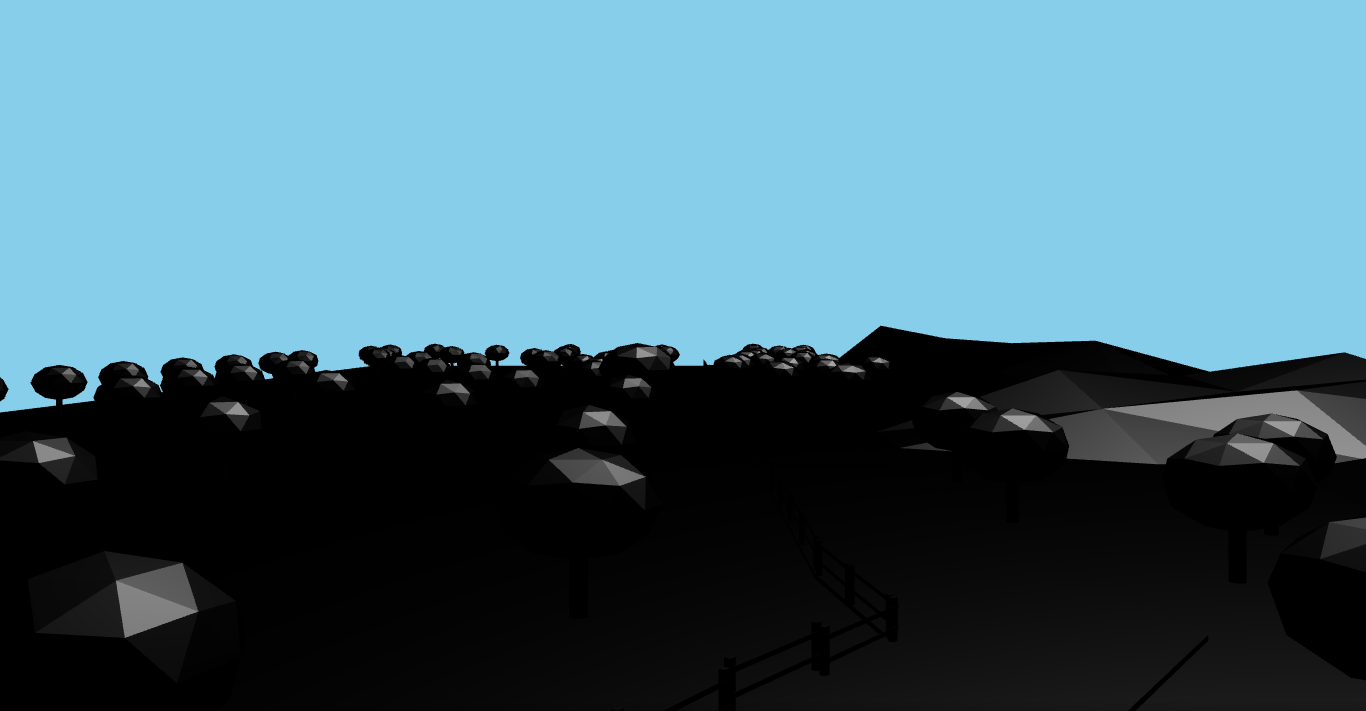
\includegraphics[width=10cm,height=10cm,keepaspectratio]{specular.png}
        \caption{Specular Lighting}
    \end{figure}
\subsection{Other graphics processing operations}
    \paragraph{Wavefront (.obj) loading}
    OBJ (or .OBJ) is a geometry definition file format first developed by Wavefront Technologies 
    for its Advanced Visualizer animation package. The file format is open and has been adopted by other 
    3D graphics application vendors.
    The OBJ file format is a simple data-format that represents 3D geometry alone — namely, the position of 
    each vertex, the UV position of each texture coordinate vertex, vertex normals, and the faces that 
    make each polygon defined as a list of vertices, and texture vertices. Vertices are stored in a 
    counter-clockwise order by default, making explicit declaration of face normals unnecessary. OBJ 
    coordinates have no units, but OBJ files can contain scale information in a human readable comment 
    line. 
    \paragraph{Texture loading}
    When texturing a mesh, you need a way to tell to OpenGL which part of the image has to be used for 
    each triangle. This is done with UV coordinates.
    Each vertex can have, on top of its position, a couple of floats, U and V. These coordinates are 
    used to access the texture. We've written a DDS file loader so as to load the texture files and feed 
    then to OpenGL texture buffer.
     DDS is a container format, it can store various types of data. However, the format is primarily used 
    to store texture data compressed with an S3 Texture Compression (S3TC) algorithm, which may be referred 
    to as a DXTn texture.  \cite{WEBSITE:1}
    The compression is a lossy compression, which means some quality is lost during the compression. 
    However, the format provides fast load times since most computer video cards natively support 
    the S3TC/DXTn compression method.

    \paragraph{Skybox Rendering}
    A cubemap is a texture that contains 6 individual 2D textures that each form one side of a cube: 
    a textured cube.\cite{WEBSITE:2} A skybox is a (large) cube that encompasses the entire scene and contains 6 images 
    of a surrounding environment, giving the player the illusion that the environment he's in is actually 
    much larger than it actually is. Some examples of skyboxes used in videogames are images of mountains, 
    of clouds, or of a starry night sky.
\subsection{Languages and tools}
    \paragraph{Language and Technologies}
    C++ was the primary language used to program the source code. C++ was used as it's one of the most popular 
    languages in the field of Graphics Programming. The community support and tutorials using C++ is tremendous. 
    To create a graphical user interface we've used the GLFW Library and GLEW was used to given OpenGL commands 
    to the Graphical Processing Unit. The whole project was build using GNU Makefile. 
    \\Specification used: OpenGL by Khronos Group
    \\Language used: C++14
    \\Build system: GNU Makefile 
    \\Graphics Library: GLFW 
    \\OpenGL Extension Library: GLEW 
    \\Version control: Git 
    \\Code hosted on: Github
    \\Assets import: Assimp library

    \paragraph{Open Asset Import Library (Assimp)}
    It is a portable Open-Source library to import various well-known 3D model formats in a uniform 
    manner. The most recent version also knows how to export 3d files and is therefore suitable as a 
    general-purpose 3D model converter.Assimp aims to provide a full asset conversion pipeline for 
    use in game engines / realtime rendering systems of any kind, but it is not limited to this purpose. 
    In the past, it has been used in a wide range of applications. Here, the whole Scene is imported as 
    an aiScene* object and the individual meshes insides are aiMesh* type objects. Each mesh inside a scene 
    is drawn after importing the whole scene using Assimp library into OpenGL. Then they were drawn individually 
    after appropriate textures were applied on them.

    \paragraph{Version Control}
    We've used Git as our version control for this project. is software for tracking changes in any set of files, 
    usually used for coordinating work among programmers collaboratively developing source code during 
    software development. It's also one of the most popular Version Control software out there and we were 
    already acquainted with Git. So, we decided to use Git as our verison controlling system. It is a free and 
    open-source system used to handle small to very large projects efficiently. We used it to tracking changes 
    in the source code.

    \paragraph{3D Modeling Software}
    Blender is a free and open-source 3D computer graphics software toolset used for creating animated films, 
    visual effects, art, 3D printed models, motion graphics, interactive 3D applications, virtual reality, 
    and computer games. Blender's features include 3D modeling, UV unwrapping, texturing, raster graphics editing, 
    rigging and skinning, fluid and smoke simulation, particle simulation, soft body simulation, sculpting, 
    animating, match moving, rendering, motion graphics, video editing, and compositing. 
\section{Result}
    After all the operations were completed and the compilation was done. We finally got the output scene on 
    the screen. We've tried to make our implementation as similar as possible to that of reference scene. 
    The camera in the scene can be controlled using Up and Down arrow keys or Right and Left Keys that allow the user 
    to move anywhere in the plane. The output scene is shown below:


\subsection{Output Images:}
\begin{figure}[h!]
      \centering
        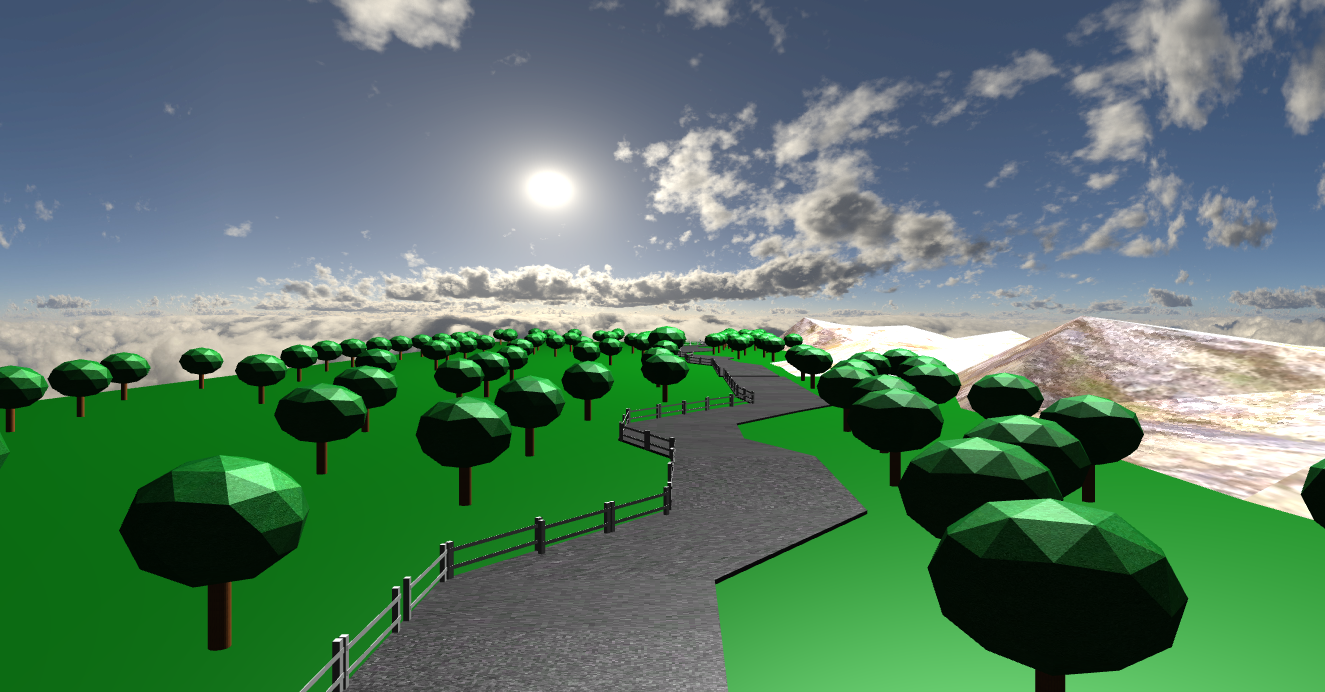
\includegraphics[width=12cm,height=12cm,keepaspectratio]{result.png}
        \caption{Final scene: Position A}
    \end{figure}
    \medskip
    \begin{figure}[h!]
      \centering
        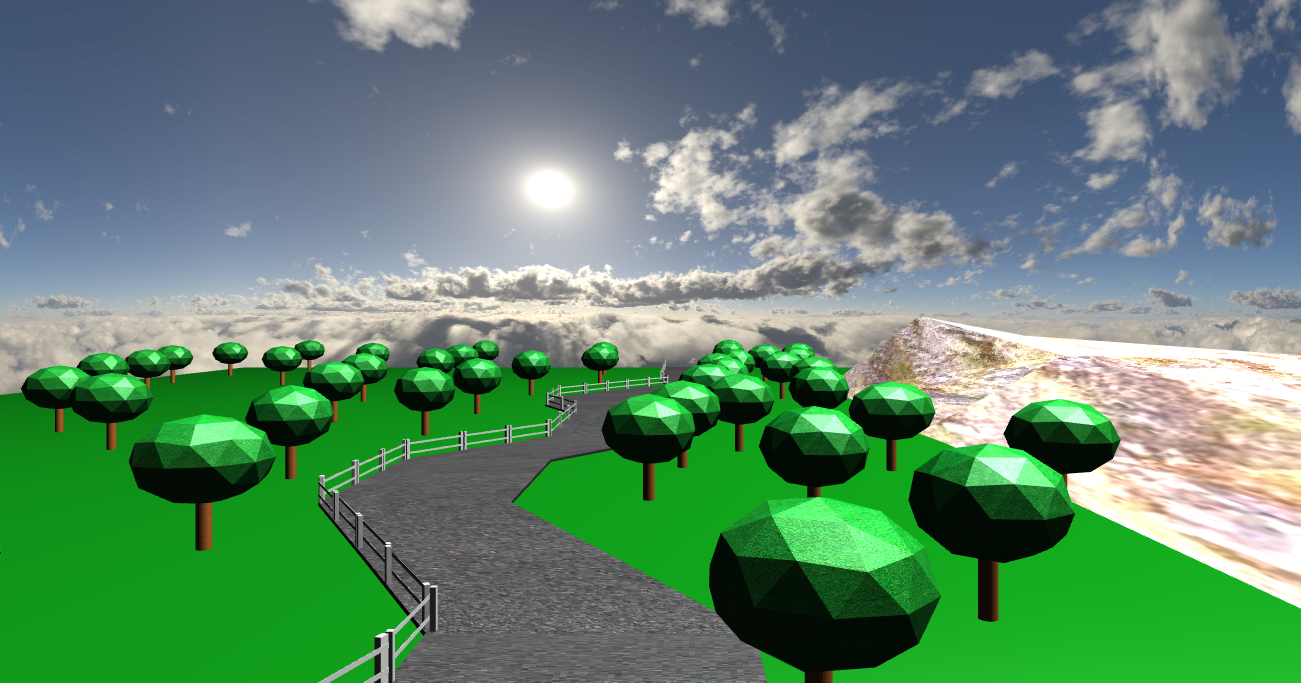
\includegraphics[width=12cm,height=12cm,keepaspectratio]{result2.png}
        \caption{Final scene: Position B}
    \end{figure}
    \medskip
\section{Conclusion}
    We learnt a lot of new things while working on this project. We started with 3D Modeling and we realized 
    that 3D Modeling requires a different set of skills than that of a Graphics Programmer. So, while working 
    in a team different tasks should be clearly assigned to each team member respective of their talents and 
    expertise. Similarly, we should always start with making our models as simple as possible and then start 
    working on making them more complex and realistic. Working with OpenGL made us realize that it can sometimes 
    be very difficult and confusing for beginners. So, proper planning and communication is essential. Since all 
    of the matrices operations will be carried out by the GPU, it is important to consider using a machine 
    that can support rendering of our models. Redundant data structures and operations should be eliminated 
    as much as possible. We also came upon the insight that things that could be automated easily such as loading 
    textures, .OBJ loading shouldn't be given more time and we should instead focus on making our Lighting, Transformations and 
    Shading implementations as robust as possible.
\section{Limitations and Future Works}
    As this was our first time trying our hands on Graphics Programming, there were many things that could've 
    been done better. We couldn't give more time to really refine our 3D Models in Blender due to lack of time. 
    The trees rendered in our demo are mostly low poly approximations. So, they're not that realistic looking. 
    Similarly, there is a lot of scope for other features. We could implement Shadow Mapping using the position 
    of Light source and the normals of Surface to display the shadows of trees on the grounds. The textures could 
    also be made more realistic but since they get extracted during UV Mapping, they started to look really 
    distorted. So, we had to settle for simple and minimalistic textures. Better depth testing algorithms could 
    be implemented so as to be more memory efficient. We're also considering adding more environment elements 
    such as grass, bushes, poles in further versions of the project.

\addcontentsline{toc}{chapter}{References}
\bibliography{graphics} 
\bibliographystyle{ieeetr}

\end{document}